% !TEX root =  ../main_manuscript.tex

\section{Results}
\label{sec:results}
From the joint model fitted to the PRIAS dataset, we found that both $\log_2 \{\mbox{PSA} + 1\}$ velocity,  and log odds of having $\mbox{DRE} > \mbox{T1c}$  were significantly associated with the hazard of cancer progression. For any patient, an increase in $\log_2 \{\mbox{PSA} + 1\}$ velocity from -0.03 to 0.16 (first and third quartiles of the fitted velocities, respectively) corresponds to a 1.94 fold increase in the hazard of cancer progression. Whereas, an increase in log odds of $\mbox{DRE} > \mbox{T1c}$ from -6.65 to -4.36 (first and third quartiles of the fitted log odds, respectively) corresponds to a 1.40 fold increase in the hazard of cancer progression. Detailed results pertaining to the fitted joint model are presented in Appendix B.

\subsection{Comparison of Various Approaches for Biopsies}
From the simulation study, we obtain the number of biopsies, and the delay in detection of cancer progression for each schedule, using ${\mbox{500} \times \mbox{250}}$ test patients. The corresponding median number of biopsies and delay are shown in Figure \ref{fig:better_balance_results}. The general trend is that more biopsies are required to have a smaller delay in detection. In addition, the personalized and PRIAS approaches seem to better balance the number of biopsies, and the delay, than the fixed/heuristic schedules. For brevity, we next detail the results for only the most widely used annual and PRIAS schedules, and compare them with personalized approach with risk thresholds of 5\% and 10\%, and threshold chosen using $\mbox{F}_1$ score. The complete set of results are presented in Appendix C.

\begin{figure}[!htb]
\captionsetup{justification=justified}
\centerline{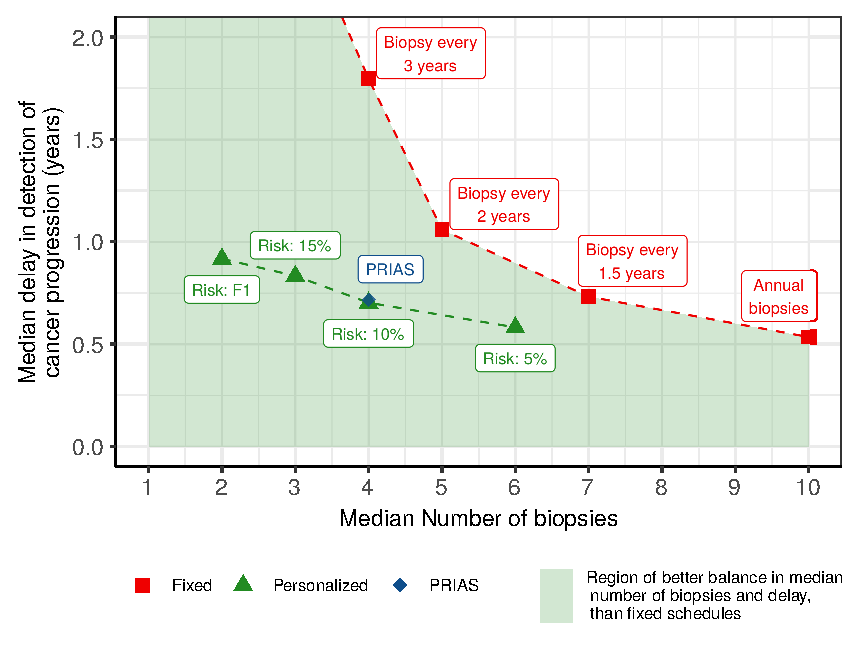
\includegraphics[width=\columnwidth]{images/better_balance_results.eps}}
\caption{\textbf{Simulation study results for burden-biopsy frontier:} Estimated median number of biopsies, and median delay in detection of cancer progression, due to the currently practiced fixed/heuristic biopsy schedules (red squares) and PRIAS schedule (blue rhombus), and personalized schedules (green triangles), over a follow-up of ten years. The green shaded region depicts the region of better balance in number of biopsies and delay, than the currently practiced fixed/heuristic schedules. Estimation is based on results obtained from the simulation study we conducted. }
\label{fig:better_balance_results}
\end{figure}

Since patients have varying cancer progression speeds, the impact of each schedule also varies with it. In order to highlight these differences we divide results for three types of patients, as per their time of cancer progression. They are \textit{fast, intermediate,} and \textit{slow progressing} patients. Although such a division may be imperfect and can only be done retrospectively in a simulation setting, we do it only for the purpose of illustration. We assume that the \textit{slow progressing} patients, are the 50\% of the total population, having a cancer progression time after the ten year follow-up period of the study (see Figure~1 in Appendix A). We assume \textit{fast progressing} patients, are the patients with an initially misdiagnosed state of cancer \cite{cooperberg2011outcomes}, or high risk patients who choose AS instead of immediate treatment. These are roughly 30\% of the population, having a cancer progression time less than 3.5 years. We label the remaining 20\% patients as \textit{intermediate progressing} patients. 

\begin{figure}[!htb]
\captionsetup{justification=justified}
\centerline{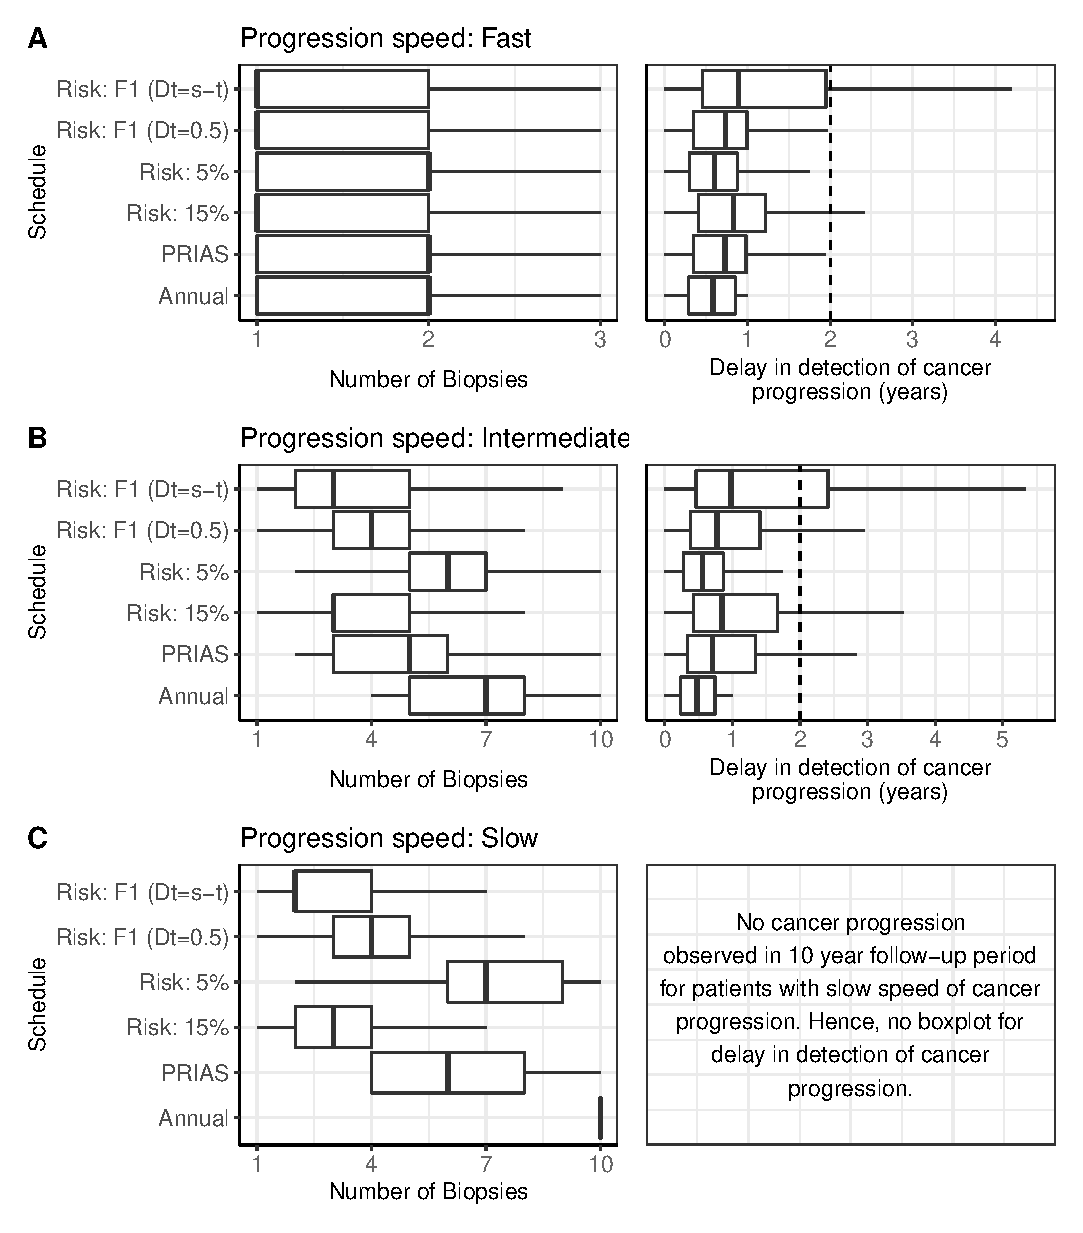
\includegraphics[width=\columnwidth]{images/sim_res_combined.eps}}
\caption{Boxplot showing variation in number of biopsies, and the delay in detection of cancer progression, in years (time of positive biopsy - true time of cancer progression) for various biopsy schedules. Biopsies are conducted until cancer progression is detected. \textbf{Panel~A:} results for simulated patients who had a faster speed of cancer progression, with progression times between 0 and 3.5 years. \textbf{Panel~B:} results for simulated patients who had an intermediate speed of cancer progression, with progression times between 3.5 and 10 years. \textbf{Panel~C:} results for simulated patients who did not have cancer progression in the ten years of follow-up. \textbf{Types of personalized schedules:} Risk:~10\% and Risk:~5\% approaches, schedule biopsy if the risk of cancer progression at a visit is more than 10\% and 5\%, respectively. Risk:~F1 works similar as previous, except that the risk threshold is chosen by maximizing $\mbox{F}_1$ score (see \hyperref[sec:methods]{Methods}). Annual corresponds to a schedule of yearly biopsies and PRIAS corresponds to biopsies as per PRIAS protocol (see \hyperref[sec:introduction]{Introduction}).}
\label{fig:sim_res_combined}
\end{figure}

The boxplots in Figure~\ref{fig:sim_res_combined}, show the variation in the number of biopsies, and the delay in detection of cancer progression, in years (time of positive biopsy - true time of cancer progression) due to various biopsy schedules, for these three types of patients. For \textit{fast progressing} patients (Panel~A,~Figure~\ref{fig:sim_res_combined}), we can see that the personalized schedules with 10\% risk and risk chosen using $\mbox{F}_1$ score, have a median of one biopsy compared to two biopsies for PRIAS and annual schedule. Despite this, the delay due to personalized schedule with 10\% risk threshold is similar to that of PRIAS schedule. 

For \textit{intermediate progressing} patients (Panel~A,~Figure~\ref{fig:sim_res_combined}), we can see that the personalized schedule with a small risk threshold of 5\% has a delay comparable to annual schedule. However, it schedules less biopsies than the annual schedule. The delay for PRIAS and personalized schedule with 10\% risk is similar, but the personalized approach schedules less biopsies comparatively for at least 50\% (median) of the patients.

The patients who are at most advantage with the personalized schedules are the \textit{slow progressing} patients (50\% of the total patients). In Panel~C of Figure~\ref{fig:sim_res_combined} we can see that the annual schedule may lead to 10 unnecessary biopsies for all such patients. The PRIAS schedule, schedules a median of 6 unnecessary biopsies. In comparison the personalized schedules using 10\% risk threshold and risk chosen using $\mbox{F}_1$ score, schedule a median of only 2 and 4 biopsies, respectively.
